\chapter{The framework}

\section{Main Scenario}

The goal is to build a platform that allows a user to query for experts in a particular domain. The
platform extracts and unifies the required information from a variety of online sources and
subsequently builds a repository of user profiles. We basically want to create a framework that would function as a Google for finding experts given a certain subject.

We will use the following steps to build such a platform:

%verduidelijken dat de volgorde van deze stappen niet belangrijk is, ze zijn interchangeable

\begin{itemize}
	%Welke auteur namen ? Waar halen we die vandaan ? Conference sites ?
	\item \textbf{Seed data} We need a list of author names to start with.
	\item \textbf{Information extraction}
		\begin{itemize}
			\item Looking up personal information, ie. profiles from LinkedIn.
			\item Looking up publications, extracting title, co-authors and affiliation. The co-authors can be used as new input for further information extraction.
			\item Categorize publications by subject
		\end{itemize}
	\item \textbf{Disambiguation} Each name is represented as a single entity. In this step we search for similarities between these entities to decide what publications belong to the same author.
\end{itemize}

A simplified representation of these steps can be seen on \ref{fig:db-gegevens}. It shows the steps that are responsible for finding the data that we will store in our database and which will be used to find experts.

\begin{figure}[htbp]
	\centering
		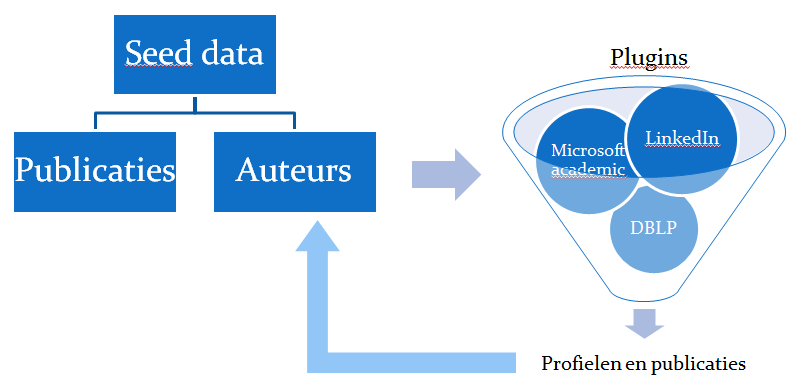
\includegraphics[width=0.75\textwidth]{fig/database-gegevens.png}
	\caption{A simplified representation of the different steps our framework takes to find data about experts.}
	\label{fig:db-gegevens}
\end{figure}

%Describe how we got to the architecture for the framework, show a figure of the (simplified + extensive) architecture and explain the different components.

\section{Features}

Based on the main scenario, we can identify a few key features our framework will need. A short summarization of each follows, explaining the challenges we face with our thesis.

%Beter verwijzen waar ze meer informatie per feature kunnen doornemen?

\subsection{Information extraction}

We need to extract information from multiple sources, which we will accomplish by using a plugin system. Each plugin is responsible for one source and will extract specific information which can be used by other plugins or other steps in our framework.

\subsection{Categorization}

In order to decide who is an expert regarding a certain subject, we will have to decide the subject of expertise of each author. A very important part of this will be in deciding the subject of the publications. The challenge is to decide this using as few information as possible, preferably by just inspecting the title, as getting access to the text of the publication itself is a whole lot more time- and resource-consuming.

\subsection{Disambiguation}

A challenging feature is the disambiguation. There are two reasons. The first is the fact that an author's name is not a unique reference for a person. There might be multiple authors with the same name, which means we have to take this into account when deciding who is an expert. Secondly, a name might be spelled differently or changed throughout time. Examples are abbreviations, an extra family name because of a marriage or simply spelling errors.

\subsection{Dynamic}

There is a big dynamic concept tied to our thesis. People who are experts on a certain subject a decade ago, may not be as important anymore now or may have changed their subject of expertise. The framework should allow new information to be processed at any time and update the expertise of authors on the flow.

\section{Architecture}

% TODO make a comparison between the first architecture we came up with and the final architecture?

Based on the scenario and the described features, we came up with the necessary components our framework needs. \ref{fig:architectuur} shows a simplistic version of how the architecture will look like. The different components of the framework and their connection toward eachother is displayed. In the next sections, the most important components will be explained at large.

% TODO : say something about the seed data and scoperfu.rb ?

\begin{figure}[htbp]
	\centering
		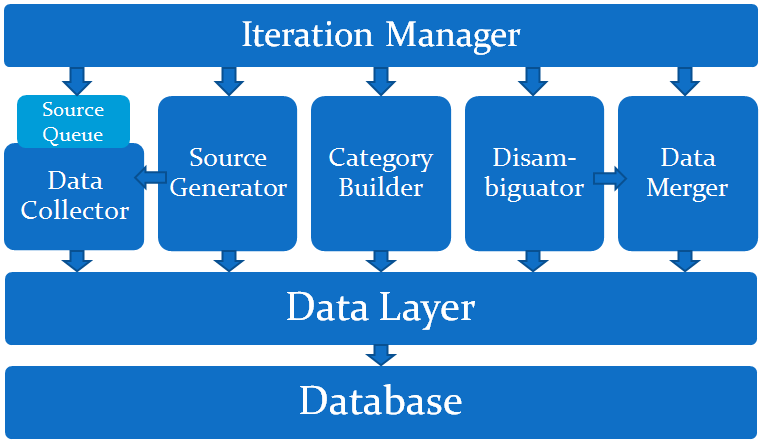
\includegraphics[width=0.75\textwidth]{fig/architectuur.png}
	\caption{First attempt at the architecture based on the necessary components}
	\label{fig:architectuur}
\end{figure}

\subsection{Iteration Manager}

This component is responsible for the flow of the entire framework. It knows what iteration our program is at and knows what the next steps are. It calls the necessary components and hands it the correct parameters in order for it to execute it's code. This will become clearer when we explain the next components.

\subsection{Data Collector}

The Data Collector receives sources from the Source Generator. It will call each of these plugins with the parameters received from the Iteration Manager, updating the database with the new data the plugins generate.

\subsection{Source Generator}

This component holds a collection of plugins, each responsible for generating data to be used by our framework coming from one source, and sends the a reference of the needed, decided by the Iteration Manager, plugins to the Source Queue in the Data Collector. 

There are different kind of plugins, according to the possible data that can be extracted. This data can include background information about a name, like location, affiliation, work experience or university. Other plugins extract information about publications (title, authors, date...) and yet another might be responsible for collecting the pdf of a publication.

%For more information about the different plugins and how they work, please refer to ??
%We want to/have set up our framework to allow new plugins to be made and used easily, extending the possibilities and usages.
% TODO : Delete this next line and either make a reference to a better explanation or better explain it here.

The different plugins we use are based on LinkedIn for personal information and DBLP en Microsoft Academic Search for bibliographic information.

% TODO : reference a plugin which is responsible for finding the pdf (something based on Google Scholar).

\subsection{Category Builder}
\label{categorybuilder}

%Category builder is eigelijk verantwoordelijk voor het opstellen van de categorie boom, zou beter zijn moest dit verantwoordelijk zijn voor het assignen van een category aan een publicatie (of een auteur?) en alles wat hier komt bij te kijken.

The Category Builder's role is deciding the subject(s) of the publications and assigning it to a category which fits in a category tree.

% TODO : Uitleg hoe dit precies in zijn werk gaat, gebruik makende van de Wikipedia API, Stanford POS Tagger.

We have two main possibilties to decide the subject of a publication. The first is by only focusing on the publication title, the second is by also making use of the actual text in the publication. The second will yield us with better results, but getting the text and analysing it will take a lot more time than just analysing a few words. 

For both manners in deciding the subject, we will make use of the Stanford Part-of-speech Tagger. We use it to select the adjectives and nouns, as these contain the most interesting information regarding to deciding the field of the publication.

When only having the publication title, the words marked by the Stanford POS Tagger will be searched on Wikipedia, by use of the API. We will search for the words seperately and make combinations, based on the closeness of the words in their original context.

% TODO : more information of HOW exactly this will work? What happens after we search them on Wikipedia ? How do we decide which ones are crap, which ones aren't ? Probably better to dedicate a whole section for the Category Builder.

When we have the original text of the publication, the easiest method is scanning for the keywords. These are often cited after the abstract and give us a very quick enumeration of the subjects discussed in the article. Another possibility is parsing the abstract itself by using the same algorithm explained above, used on the publication title.


\subsection{Disambiguator}
\label{disambiguator}

The disambiguation is an important factor towards the strength of our framework. In the data collection phase, we view each name as e new object in our database, even if that name is already stored. This is necessairy to keep the option open that the same name might be connected towards different authors. This also means our database grows fast. 

The disambiguation exists out of a number of rules. These inspect several objects in the database and define the probabilities that names, typically connected to a publication or a profile, are connected to eachother and to one author. %These probabilities are stored as weights of edges between these objects.

An in-depth explanation of these rules can be found in \ref{disamb_rules}.

\subsection{Data Merger}

The Data Merger is responsible for merging the names together so they would reference to the same author. This component uses the probabilities calculated by the Disambiguator in order to do so.

%\section{Technologies}
%
%\subsection{MySQL}
%
%Discuss the differences, advantages and disadvantages between a relational datastore, a record-store and a triple-store.
%
%\subsubsection{Relational datastore}
%
%\subsubsection{A record-store}
%
%\subsubsection{Triple-store}
%
%\subsubsection{Conclusion}
%
%We choose to use MySQL, a relational datastore, because we are familiar with it. It allows us to quickly set up our prototype to work and test our framework on.
%
%\subsection{Two databases}
%
%We use two databases, one for development and one for production.
%
%The former is used to collect all information about the possible experts and their work. 
%
%\subsection{Ruby}
